\documentclass[12pt,a4paper]{article}
\usepackage[polish]{babel}
\usepackage[T1]{fontenc}
\usepackage[utf8x]{inputenc}
\usepackage{hyperref}
\usepackage{url}
\usepackage{graphicx}
\usepackage{algorithm2e}
\usepackage{capt-of}

\usepackage{color}
\usepackage{listings}

\lstloadlanguages{% Check Dokumentation for further languages ...
	C,
	C++,
	Java,
	Python
}

\definecolor{red}{rgb}{0.6,0,0} % for strings
\definecolor{blue}{rgb}{0,0,0.6}
\definecolor{green}{rgb}{0,0.8,0}
\definecolor{cyan}{rgb}{0.0,0.6,0.6}

\lstset{
	language=csh,
	basicstyle=\footnotesize\ttfamily,
	numbers=left,
	numberstyle=\tiny,
	numbersep=5pt,
	tabsize=2,
	extendedchars=true,
	breaklines=true,
	frame=b,
	stringstyle=\color{blue}\ttfamily,
	showspaces=false,
	showtabs=false,
	xleftmargin=17pt,
	framexleftmargin=17pt,
	framexrightmargin=5pt,
	framexbottommargin=4pt,
	commentstyle=\color{green},
	morecomment=[l]{//}, %use comment-line-style!
	morecomment=[s]{/*}{*/}, %for multiline comments
	showstringspaces=false,
	morekeywords={ abstract, event, new, struct,
		as, explicit, null, switch,
		base, extern, object, this,
		bool, false, operator, throw,
		break, finally, out, true,
		byte, fixed, override, try,
		case, float, params, typeof,
		catch, for, private, uint,
		char, foreach, protected, ulong,
		checked, goto, public, unchecked,
		class, if, readonly, unsafe,
		const, implicit, ref, ushort,
		continue, in, return, using,
		decimal, int, sbyte, virtual,
		default, interface, sealed, volatile,
		delegate, internal, short, void,
		do, is, sizeof, while,
		double, lock, stackalloc,
		else, long, static,
		enum, namespace, string},
	keywordstyle=\color{cyan},
	identifierstyle=\color{red},
}
\usepackage{caption}
\DeclareCaptionFont{white}{\color{white}}
\DeclareCaptionFormat{listing}{\colorbox{blue}{\parbox{\textwidth}{\hspace{15pt}#1#2#3}}}
\captionsetup[lstlisting]{format=listing,labelfont=white,textfont=white, singlelinecheck=false, margin=0pt, font={bf,footnotesize}}

\addtolength{\hoffset}{-1.5cm}
\addtolength{\marginparwidth}{-1.5cm}
\addtolength{\textwidth}{3cm}
\addtolength{\voffset}{-1cm}
\addtolength{\textheight}{2.5cm}
\setlength{\topmargin}{0cm}
\setlength{\headheight}{0cm}

\title{\textbf{Dokumentacja Projektu\\ Program Liczb Zaprzyjaźnionych}}
\author{\\Natalia Szalas\\ Informatyka, sem. III, gr. 2D\\Wydział Matematyki Stosowanej}
\date{15 Stycznia 2021}

\begin{document}

\maketitle
\newpage
\tableofcontents

\newpage
	\section{Część I}
	\subsection{Treść zadania: Liczby zaprzyjaźnione}
	\hspace{20} Za Wikipedią: Liczby zaprzyjaźnione to para różnych liczb naturalnych, takich, że suma dzielników każdej z tych liczb równa się drugiej (nie uwzględniając tych dwóch liczb jako dzielników). Np. liczba 284 ma dzielniki: 1, 2, 4, 71, 142, których suma daje 220, a liczba 220 ma dzielniki: 1, 2, 4, 5, 10,11, 20, 22, 44, 55, 110, których suma daje 284. Zatem liczby 220 i 284 tworzą, parę liczb zaprzyjaźnionych. Należy napisać program, który dla dowolnej pary różnych liczb naturalnych będzie rozstrzygał, czy para ta tworzy liczby zaprzyjaźnione. \newline
	
	\subsection{Opis programu}
	\hspace{20} Program ma na celu ustalenie czy dwie liczby są zaprzyjaźnione. Oznacza to, że suma wszystkich dzielników pierwszej liczby, musi się równać drugą liczbę. Przykład: jeśli mamy liczby 220 oraz 284:
	\begin{itemize}
	    \item 220 = 1 + 2 + 4 + 71 + 142 (dzielniki 284)
	    \item 284 = 1 + 2 + 4 + 5 + 10 + 11 + 20 + 22 + 44 + 55 + 110 (dzielniki 220) \newline
	\end{itemize}
	
	\subsection{Pseudokod}
	
	\begin{algorithm}[H]
	\SetAlgoLined
	\KwData{num1, num2, areFriends(), sumDivisors()}{}
	\KwResult{Sprawdzenie czy liczby są zaprzyjaźnione }
	 {funkcja areFriends()}\;
	 \eIf {num1 != num2}{
	   \eIf{num1 == sumDivisors(num2) && num2 == sumDivisors(num1)}{
	   liczby są zaprzyjaźnione}{
	   liczby nie są zaprzyjaźnione}\;
	 }
	 {
	 numery są takie same, wiec nie można ich porównać}\;
  

\end{algorithm}

\newpage
	\subsection{Instrukcja obsługi i działania}
	\hspace{20} Po uruchomieniu aplikacji pojawia się menu z opcjami do wyboru:
	\begin{enumerate}
	   
	    \item Uruchom program  - uruchamia plik .py, zwraca 2 pliki .txt
	    \item Wykonaj podsumowanie  - uruchamia plik .py, zwraca html
	    \item Informacje o działaniu 
	    \item Backup  - tworzy kopię zapasową
	    \item Zakoncz - kończy prace programu
	    
	\end{enumerate}
	
	\begin{figure}[h]
	    \begin{center}
	    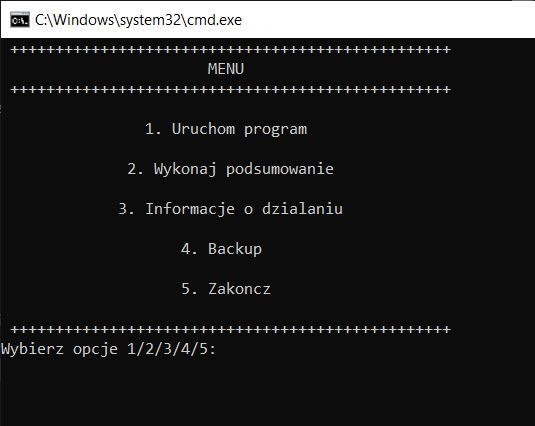
\includegraphics[width=10cm]{menu.JPG}
	    \caption{Przykład menu}
	    \end{center}
	    \end{figure}
	
	
	\hspace{10} W celu uzyskania rezultatów, należy najpierw odpowiednio napisać plik tekstowy. Oznacza to, że każda para liczb musi znajdować się w osobnej linijce. Do tego trzeba oddzielić je spacją oraz dodać spację za drugą liczbą. (rys.2) \newline
	
	\begin{center}
	    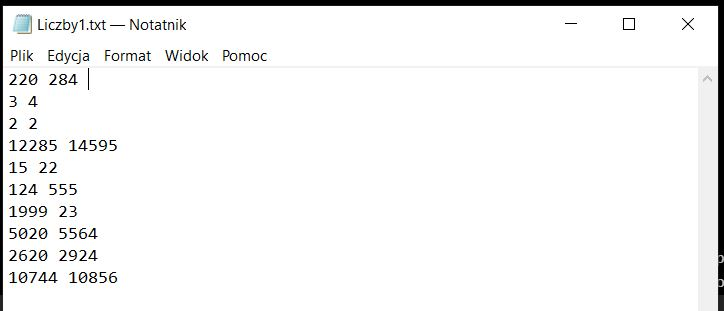
\includegraphics[]{input.JPG}
	    \begin{caption}
	    \caption{Rysunek 2: Przykład pliku wejściowego}
	    \end{caption}
	    \end{center}
    	
    	
	
	\hspace{10} Przy wyborze opcji numer 1, po wpisaniu nazwy pliku, rozpocznie się proces sprawdzania czy liczby są zaprzyjaźnione, a jego rezultaty zostaną zapisane do pliku tekstowego(rys.3). W tym samym czasie wykona się statystyka, która również pojawi się w pliku txt(rys.4).
	
	    \begin{center}
	    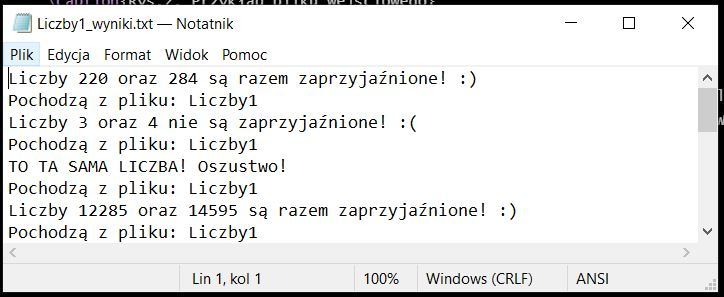
\includegraphics[width=17cm]{wyniki.JPG}
	    \begin{caption}
	    \caption{Rysunek 3: Plik tekstowy z wynikami}
	    \end{caption}
	    \end{center}
	    

	    \begin{center}
	    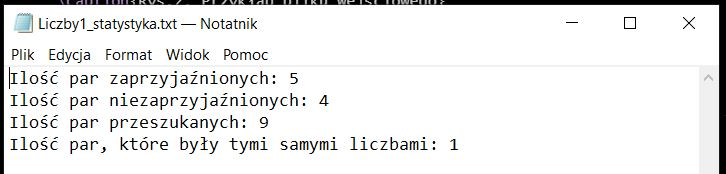
\includegraphics[width=17cm]{statystyka.JPG}
	    \begin{caption}
	    \caption{Rysunek 4: Plik tekstowy ze statystyką}
	    \end{caption}
	    
	    \end{center}
	    
	
	\hspace{10} \\  \\ Przy opcji numer 2, po wpisaniu odpowiedniej nazwy, rozpocznie się przetwarzanie danych z wyniki.txt oraz statystyka.txt, w wyniku którego utworzy się strona HTML z jasnym raportem na temat interesującego nas tematu(rys.5). \\
	
	    \begin{center}
	    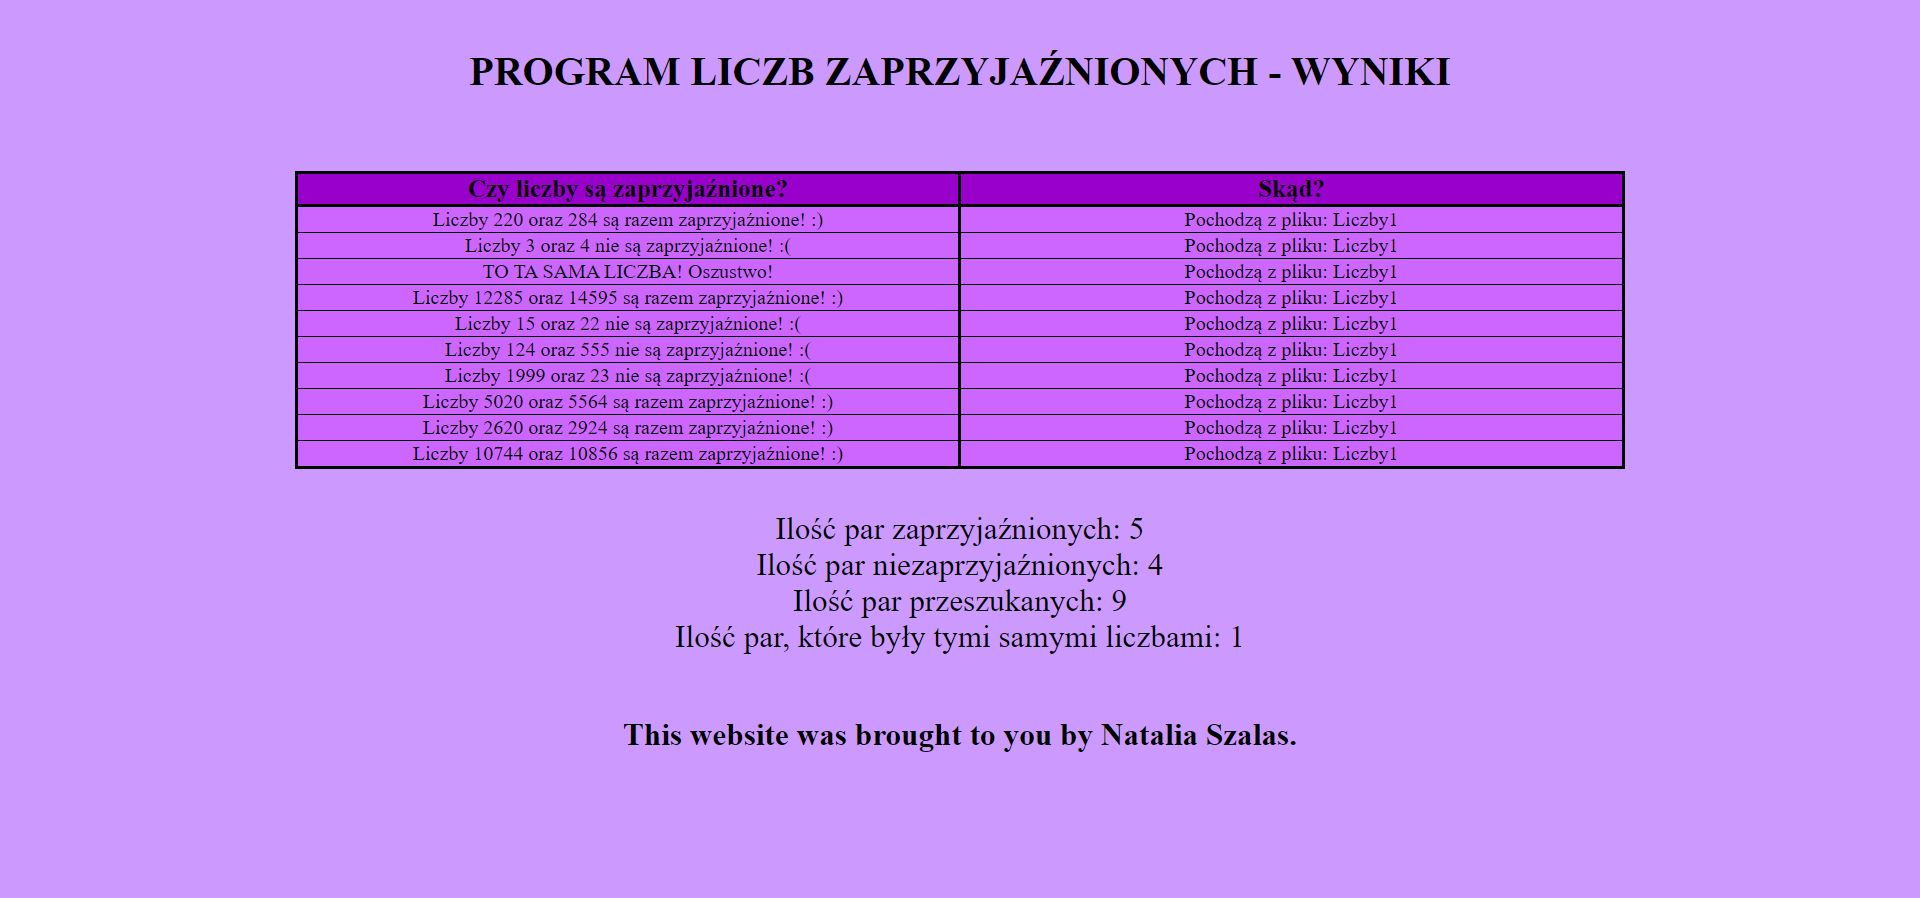
\includegraphics[width=17cm]{strona.JPG}
	    \begin{caption}
	    \caption{Rysunek 5: Strona HTML}
	    \end{caption}
	    \end{center}
	    
	
	\hspace{10}\\ \\ Przy opcji numer 3, otworzą się informacje odnośnie programu. \\ Przy opcji numer 4 utworzy się kopia zapasowa w osobnym pliku zwanym backup. \\ Opcja numer 5 zakończy działanie programu i zamknie okienko.
	
	\newpage
	\subsection{Schematy blokowe wybranych funkcji} 
	
	
	    \begin{center}
	    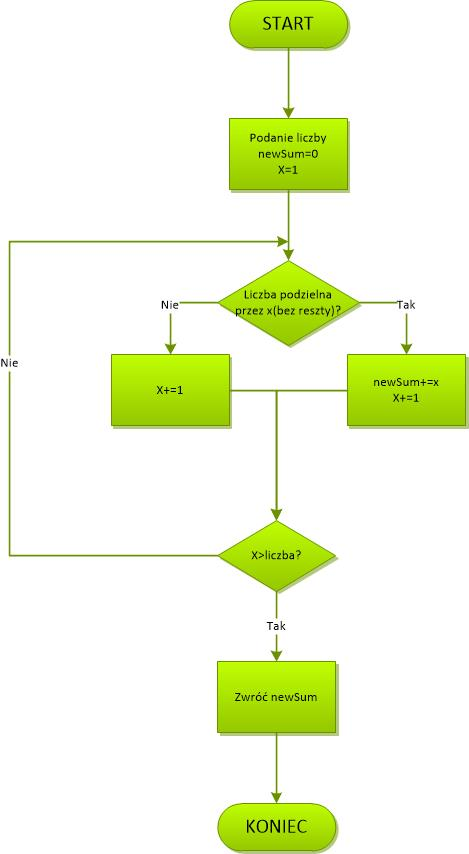
\includegraphics[]{sumDivisors.jpg}
	    \newline \newline
	    \begin{caption}
	    \caption{Rysunek 6: Funkcja sumDivisors()}
	    \end{caption}
	    
	    \end{center}
	    
	    
	\newpage
	
	    \begin{center}
	    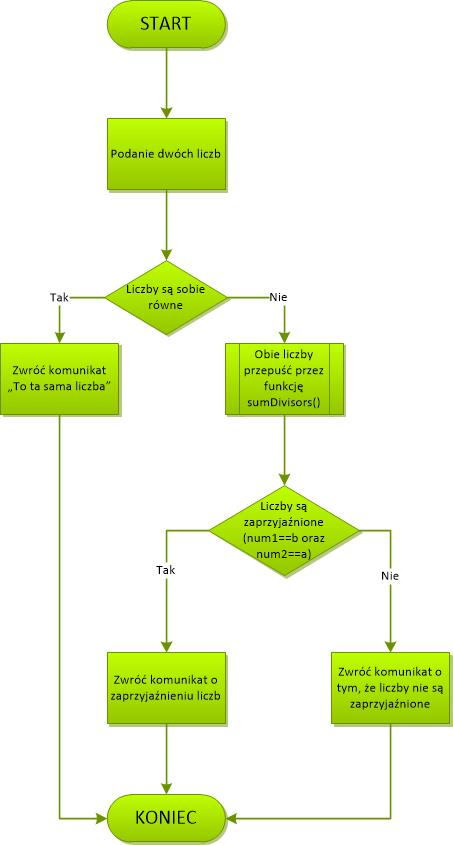
\includegraphics[height = 17cm]{areFriends().jpg}
	    \newline \newline
	    \begin{caption}
	    \caption{Rysunek 7: Funkcja areFriends()}
	    \end{caption}
	    \end{center}
	    
	    
	\newpage
	
	    \begin{center}
	    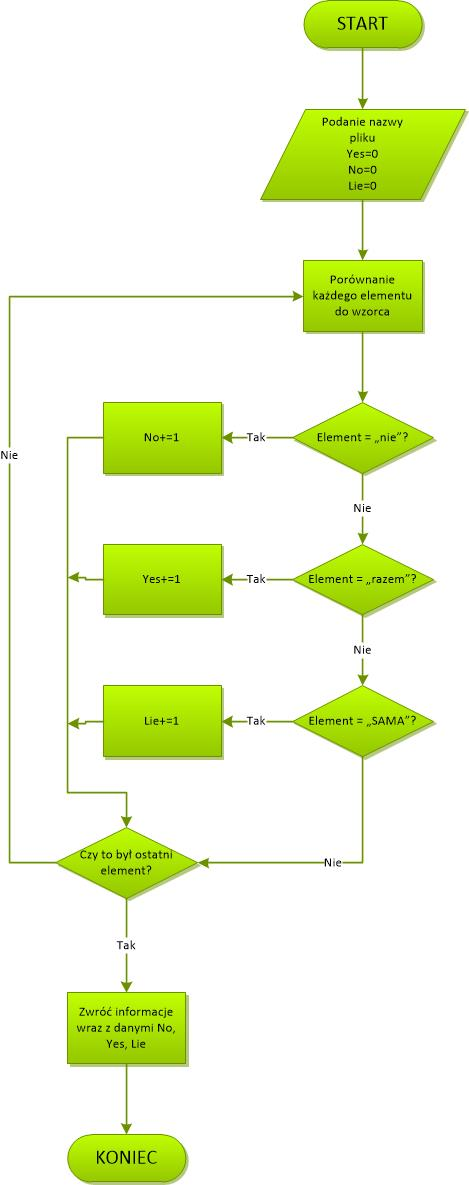
\includegraphics[height = 20cm]{statistics.jpg}
	    \newline \newline
	    \begin{caption}
	    \caption{Rysunek 8: Funkcja statistics()}
	    \end{caption}
	    
	    \end{center}
	    

	\newpage
	\begin{figure}[h]
	    \begin{center}
	    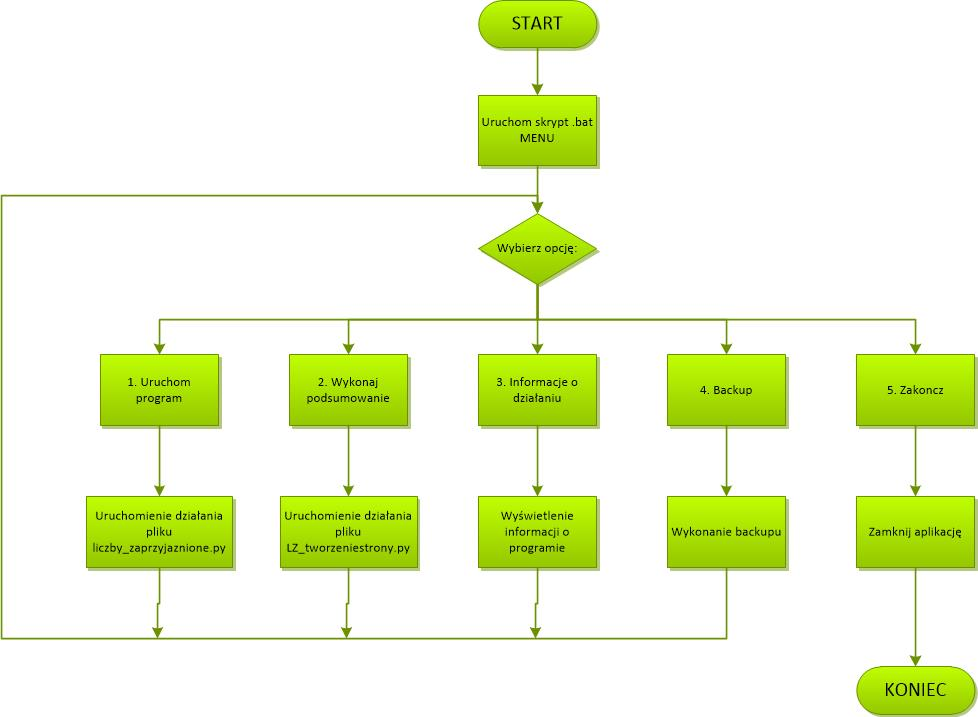
\includegraphics[width = 18cm]{dzialanieMenu.jpg}
	    \caption{Schemat działania Menu z pliku .bat}
	    \end{center}
	    \end{figure}
	\newpage
	\section{Część II}
	\subsection{Część techniczna}
	\hspace{20} Program składa się z plików: .bat, .py, .txt oraz .html. Po uruchomieniu pliku bat, wchodzimy w opcję pierwszą. Wówczas uruchamia się plik liczby\_zaprzyjaznione.py, zawierający cały algorytm: \\ \\
	Po wprowadzeniu nazwy pliku do sprawdzenia, uruchamia się funkcja LoadFile() wyszukująca danych do pobrania. Gdy operacja przejdzie pomyślnie, dane są dzielone w odpowiedni sposób do dalszej obróbki. Następnie uruchamia się funkcja areFriends(), w której na podanych dwóch liczbach sprawdza się warunki bycia zaprzyjaźnionymi. W środku znajdziemy również funkcję sumDivisors(), która w szybki sposób oblicza sumę dzielników danej liczby. Później uzyskane rezultaty zapisują się do pliku tekstowego za pomocą funkcji SaveFile(). Na sam koniec tworzy się również plik statystyk zliczający ilość odpowiednich słów i zwracający uzyskane rachunki w postaci pliku txt.\\ \\
	Kolejnym procesem jest pełen raport uzyskany z opcji numer dwa w menu, który analizując pliki txt, zwraca plik html. \\ \\ 
	
	\begin{center}
	    \subsection{PLIKI PROJEKTU}
	\end{center}
	
	\begin{itemize}
	    \item Projekt
	    \begin{itemize}
	        \item liczby\_zaprzyjaznione.bat
	        \item liczby\_zaprzyjaznione.py
	        \item Liczby1.txt
	        \item Liczby1\_statystyka.txt
	        \item Liczby1\_wyniki.txt
	        \item Liczby1\_zaprzyjaznione.html
	        \item Liczby2.txt
	        \item LZ\_tworzeniestrony.py
	    \end{itemize}
	    \item Dokumentacja
	    \begin{itemize}
	        \item Dokumentacja.pdf
	        \item Grafiki(folder)
	    \end{itemize}
	    \item backup
	\end{itemize}
	
	\newpage
	\section{PODSUMOWANIE}
	\subsection{Raport ogólny}
	\hspace{20} Program działa poprawnie i zgodnie z przeznaczeniem. Został napisany w systemie operacyjnym Microsoft Windows 10 Home, a jego część python'owska w Visual Studio Code. Aplikacja nie była testowana w systemie Linux. \\ Zadanie z powyższym algorytmem pochodzi z konkursu 'Algorytmion' z roku 2013.\\ \\
	Nie udało się zrealizować odczytu plików z osobnego folderu, ani zapisu plików do innego folderu niż ten, w którym znajdują się wszystkie pliki .bat oraz .py.
	\subsection{Propozycje ulepszeń}
	\hspace{20} Program nie został napisany w celach komercyjnych, jednak gdyby chcieć go sprzedać, należałoby popracować nad oprawą graficzną. Można również stworzyć ulepszenia w postaci automatycznego backupu co miesiąc oraz dodatkowych funkcji, bądź dopisania kilku innych algorytmów. W ten sposób powstałaby aplikacja Algus, która miałaby więcej niż jeden cel. Warto by również umniejszyć wkład użytkownika, w intencji wykazywania mniejszej ilości błędów.
   \newpage
   \begin{center}
       \subsection*{PEŁEN KOD PROGRAMU}
   \end{center}
   \begin{itemize}
       \item liczby\_zaprzyjaznione.bat
       \begin{lstlisting}
           @echo off 

goto MENU
:MENU
cls
echo  +++++++++++++++++++++++++++++++++++++++++++++++++
echo                        MENU                      
echo  +++++++++++++++++++++++++++++++++++++++++++++++++
echo.                                   
echo                 1. Uruchom program                    
echo.                                   
echo               2. Wykonaj podsumowanie                
echo.
echo              3. Informacje o dzialaniu 
echo.                                 
echo                     4. Backup                  
echo.                                
echo                     5. Zakoncz                  
echo.                               
echo  +++++++++++++++++++++++++++++++++++++++++++++++++

set /p wybor="Wybierz opcje 1/2/3/4/5: "
If %wybor%==1 goto URUCHOM
If %wybor%==2 goto ZACZNIJ
If %wybor%==3 goto INFO
If %wybor%==4 goto BACKUP
If %wybor%==5 goto exit

:URUCHOM
cls
liczby_zaprzyjaznione.py
set /p wybor="Aby wrocic do MENU nacisnij ENTER..."
goto MENU

:ZACZNIJ
cls
LZ_tworzeniestrony.py
set /p wybor="Aby wrocic do MENU nacisnij ENTER..."
goto MENU

:INFO
cls
echo  +++++++++++++++++++++++++++++++++++++++++++++++++
echo               INFORMACJE O PROGRAMIE
echo  +++++++++++++++++++++++++++++++++++++++++++++++++
echo.
echo   Glownym celem programu jest sprawdzenie czy
echo   suma wszystkich dzielnikow pierwszej z liczb 
echo   rowna sie liczbie drugiej i na odwrot. 
echo.
echo   Aby program poprawnie zadzialal, kazda para 
echo   liczb musi znajdowac sie w osobnej linijce pliku
echo   tekstowego. Do tego liczby musza zostac 
echo   oddzielone spacja, ktora musi tez zostac dodana 
echo   za druga z nich. 
echo.
echo   Istnieje rowniez funkcja "Wykonaj podsumowanie"
echo   wyswietlajaca wyniki dla wczesniej uruchomionego 
echo   programu w postaci strony HTML.
echo.
echo.
echo   Program napisany przez Natalie Szalas.
echo.
echo.  
set /p wybor="Aby wrocic do MENU nacisnij ENTER..."
goto MENU


:BACKUP
set Day=%Date:~0,2%
set Mth=%Date:~3,2%
set Yr=%Date:~6,4%
set Hour=%Time:~0,2%
if "%hour:~0,1%" == " " set hour=0%hour:~1,1%
set Min=%Time:~3,2%
set name="%date%-%hour%.%min%"

cd..
mkdir "backup\%name%"
xcopy Projekt backup\%name% /E /I /H /Y

cls
echo  +++++++++++++++++++++++++++++++++++++++++++++++++
echo                        BACKUP                      
echo  +++++++++++++++++++++++++++++++++++++++++++++++++
echo.
echo.
echo   Backup zostal wykonany z data %name%
echo.
echo.
echo  +++++++++++++++++++++++++++++++++++++++++++++++++
echo.
set /p wybor="Aby wrocic do MENU nacisnij ENTER..."
goto MENU

       \end{lstlisting}
       \item liczby\_zaprzyjaznione.py
	\begin{lstlisting}
	    import sys,os

def sumDivisors(number):
    newSum = 0
    for x in range(1, number):
        if number%x == 0:
            newSum+=x
        else:
            continue
    return newSum

def areFriends(num1,num2):
    k=""
    if num1!=num2:
        a=sumDivisors(num1)
        b=sumDivisors(num2)
        if num1==b and num2==a:
            k="Liczby "+str(num1)+" oraz "+ str(num2)+" sa razem zaprzyjaznione! :)"
        else:
            k="Liczby "+str(num1)+" oraz "+str(num2)+" nie sa zaprzyjaznione! :("
    else:
       k = "TO TA SAMA LICZBA! Oszustwo!"
    
    return k

def LoadFile(fol):
    dirname = os.path.dirname(__file__)
    filename = os.path.join(dirname, fol)
    text=""
    try:
        folder=open(filename,"r")
        text = folder.readlines()    
    except IOError:
        print("Blad przy probie otworzenia pliku!")
        print(filename)
        exit() 
    return text

def SaveFile(czyzap, fileName):
    fil = open(fileName+"_wyniki.txt", "a")
    fil.write(str(czyzap))
    fil.write("\nPochodza z pliku: "+fileName+"\n")
    fil.close()

def statistics(fileName):
    yes = 0
    no = 0
    lie = 0
    newName=fileName+"_wyniki.txt"
    fol = LoadFile(newName)
    fol1=[]
    for n in range(0,len(fol)):
        fol1+=fol[n].split(" ")

    #fol1=fol.split("\w ")
    for x in range(0, len(fol1)):
        if fol1[x]=="nie":
            no+=1
        if fol1[x]=="razem":
            yes+=1
        if fol1[x]=="SAMA":
            lie+=1
        else:
            continue
    
    naTak = "Ilosc par zaprzyjaznionych: "+str(yes)
    naNie = "Ilosc par niezaprzyjaznionych: "+str(no)
    together = "Ilosc par przeszukanych: "+str((yes+no))
    oszustwa = "Ilosc par, ktore byly tymi samymi liczbami: "+str(lie)
    saveName = fileName+"_statystyka.txt"
    k = open(saveName, "w")
    k.write(naTak+"\n"+naNie+"\n"+together+"\n"+oszustwa)


l = input("Podaj nazwe pliku bez jego rozszerzenia: ")
test = LoadFile(l+".txt")
for x in range(0,len(test)):
    luv = test[x].split(" ")
    c = int(luv[0])
    d = int(luv[1])
    kap=areFriends(c,d)
    SaveFile(kap, l)
statistics(l)





	\end{lstlisting}
	
	\item LZ\_tworzeniestrony.py
	\begin{lstlisting}
	    import webbrowser

l = input("Podaj poczatek nazwy pliku az do _wynik.txt: ")
z = l+"_wyniki.txt"
n = l+"_statystyka.txt"
name=l+"_zaprzyjaznione.html"
f = open(name,'w')
table=" "
i=0

#Generowanie tabeli
try:
    plik = open(z)
    for line in plik:
        if(i%2==0):
            table += """<tr>"""
        table+="""<td>"""+line
        i+=1
except IOError:
    print("Blad otwarcia pliku!")
    exit()

#Wczytywanie statystyk
try:
    stat = open(n)
    statystyka="""<h4>"""
    for line in stat:
        statystyka+=line+"""<br>"""
    statystyka+="""</h4>"""
except IOError:
    print("Blad otwarcia pliku!")
    exit()

#Budowa strony
ttop="""
<table>
   <thead>
      <tr> <th> Czy liczby sa zaprzyjaznione? <th> Skad? 
   <tbody>
"""

top = """
<html>
<center>
<style>
body {background-color: CC99FF;}
h1 {padding: 30px;padding-bottom: 40px;}
th, td, table {border: 1px solid black}
th{width: 33%;}
table{background-color:#CC66FF; margin-bottom:15px;}
thead tr, thead th{border: 3px solid black; font-size: 20px;background-color:#9900CC; witdh: 33%;}
td {border-left: 3px solid black;}
table {width: 70%; border-collapse: collapse; text-align: center; border: 3px solid black}
h3 {text-align:center; margin-top: 50px; font-size: 25px}
h4 {text-align:center; font-weight: normal; font-size: 25px}
</style>
<head><h1>PROGRAM LICZB ZAPRZYJAZNIONYCH - WYNIKI </h1></head>
<body>
"""

tend = """
</table>
"""

bottom = """
<h3>This website was brought to you by Natalia Szalas.</h3.	
</body>
</center>
</html>
"""

#Generowanie calosci
f.write(top+ttop+table+tend+statystyka+bottom)
f.close()
	\end{lstlisting}
	\end{itemize}

   

\end{document}
